\documentclass{article}
\usepackage{include/nips13submit_e,times}
%%%%%%%%%%%%%%%%%%%%%%%%%%%%%%%%%%%%%%%%%%%%%%%%%%%%%%%%%%%
%%%% EDITING HELPER FUNCTIONS  %%%%%%%%%%%%%%%%%%%%%%%%%%%
%%%%%%%%%%%%%%%%%%%%%%%%%%%%%%%%%%%%%%%%%%%%%%%%%%%%%%%%%%

%% NA: needs attention (rough writing whose correctness needs to be verified)
%% TBD: instructions for how to fix a gap ("Describe the propagation by ...")
%% PROBLEM: bug or missing crucial bit 

%% use \fXXX versions of these macros to put additional explanation into a footnote.  
%% The idea is that we don't want to interrupt the flow of the paper or make it 
%% impossible to read because there are a bunch of comments.

%% NA's (and TBDs, those less crucially) should be written so 
%% that they flow with the text.

\definecolor{WowColor}{rgb}{.75,0,.75}
\definecolor{SubtleColor}{rgb}{0,0,.50}

% inline
\newcommand{\NA}[1]{\textcolor{SubtleColor}{ {\tiny \bf ($\star$)} #1}}
\newcommand{\LATER}[1]{\textcolor{SubtleColor}{ {\tiny \bf ($\dagger$)} #1}}
\newcommand{\TBD}[1]{\textcolor{SubtleColor}{ {\tiny \bf (!)} #1}}
\newcommand{\PROBLEM}[1]{\textcolor{WowColor}{ {\bf (!!)} {\bf #1}}}

% as margin notes

\newcounter{margincounter}
\newcommand{\displaycounter}{{\arabic{margincounter}}}
\newcommand{\incdisplaycounter}{{\stepcounter{margincounter}\arabic{margincounter}}}

\newcommand{\fTBD}[1]{\textcolor{SubtleColor}{$\,^{(\incdisplaycounter)}$}\marginpar{\tiny\textcolor{SubtleColor}{ {\tiny $(\displaycounter)$} #1}}}

\newcommand{\fPROBLEM}[1]{\textcolor{WowColor}{$\,^{((\incdisplaycounter))}$}\marginpar{\tiny\textcolor{WowColor}{ {\bf $\mathbf{((\displaycounter))}$} {\bf #1}}}}

\newcommand{\fLATER}[1]{\textcolor{SubtleColor}{$\,^{(\incdisplaycounter\dagger)}$}\marginpar{\tiny\textcolor{SubtleColor}{ {\tiny $(\displaycounter\dagger)$} #1}}}

\usepackage{include/preamble}


\title{A Nonparametric Model of Censoring}


\author{
Pittsburgh, PA 15213 \\
\texttt{hippo@cs.cranberry-lemon.edu} \\
\And
Coauthor \\
Affiliation \\
Address \\
\texttt{email} \\
\AND
Coauthor \\
Affiliation \\
Address \\
\texttt{email} \\
}

% The \author macro works with any number of authors. There are two commands
% used to separate the names and addresses of multiple authors: \And and \AND.
%
% Using \And between authors leaves it to \LaTeX{} to determine where to break
% the lines. Using \AND forces a linebreak at that point. So, if \LaTeX{}
% puts 3 of 4 authors names on the first line, and the last on the second
% line, try using \AND instead of \And before the third author name.

\newcommand{\fix}{\marginpar{FIX}}
\newcommand{\new}{\marginpar{NEW}}

%\nipsfinalcopy % Uncomment for camera-ready version

\begin{document}


\maketitle

\begin{abstract}
Data-dependent non-response is one of the central problems of statistical inference.  We introduce a nonparametric density model capabale of inferring both censored distributions, and a model of the censoring process.  This is acheived through the use of a novel inference scheme: ``exact-approximate'' Hamiltonian Monte Carlo.  We demonstrate our model on toy datasets as well as cool real problems.
\end{abstract}

\section{Introduction}

[Discuss censoring, truncation, data-dependent non-response]

[Give several examples: surveys, government censorship, faulty sensors]

[Briefly discuss previous approaches]

We introduce a generative non-parametric model to address this problem.  Our approach is based on the GP-LVM ~\cite{lawrence2004gaussian,salzmann2008local,lawrence2009non}, a flexible nonparametric density model.

This model is a natural problem with which to demonstrate recent advances in ``exact-approximate'' Monte Carlo methods, which allow one to construct valid Markov chains with only approximate evaluations of the likelihood function.

\section{Censoring problems}

In this section, we give a formal definition of censoring and truncation.

Food for thought: If data is truncated, but we know its marginal distribution, would that be more accurately described as censoring, since we do know that the data is there?

[Cite Ben Marlin's thesis. Discuss how people usually assume that the non-response is independent of the data to allow simple inference schemes, but that this is usually unrealistic]

Examples: 




\section{The Censored GP-LVM}

In this section, we define in detail the actual model.

\subsection{Gaussian Process Latent Variable Model}

\begin{figure}
\centering
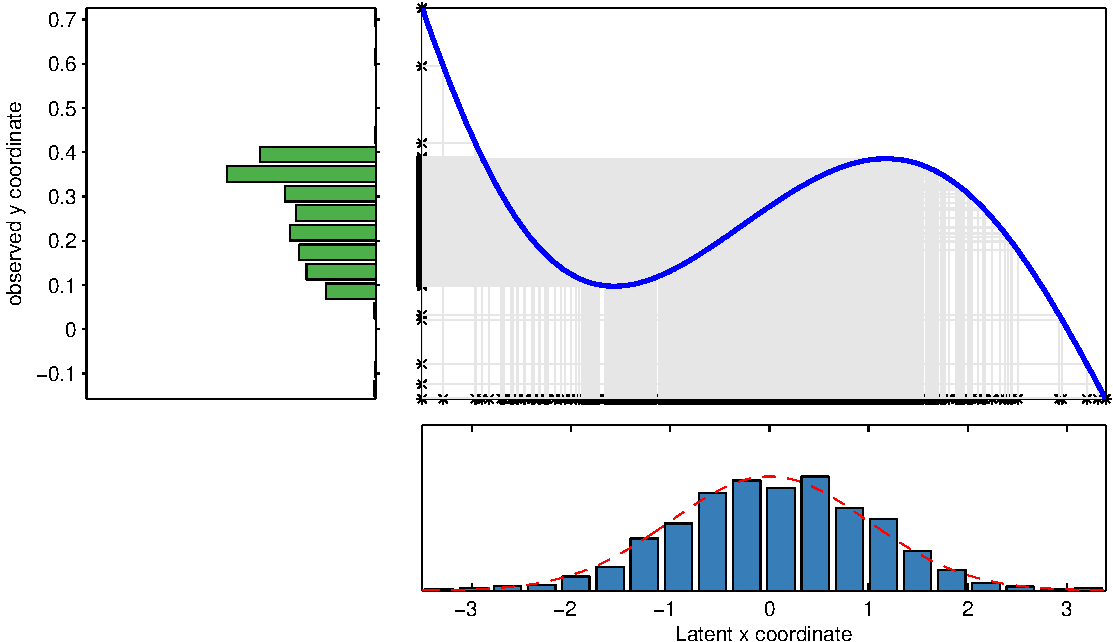
\includegraphics[width=0.8\columnwidth]{figures/gplvm_1d_draw_8} 
\caption{A draw from a Gaussian process latent variable model.  Bottom:  The latent datapoints $\vX$ are distributed according to a parametric base distribution (a Gaussian).  Top right:  A smooth function $f$ drawn from a Gaussian process prior is applied to obtain $\vY$ = $f(\vX)$.  Left:  The observed data $\vY$ is distributed according to a non-Gaussian density.}
\label{fig:gplvm_intro}
\end{figure}

The GP-LVM specifies a model wherein latent variables $\vX$ are warped by an unknown smooth, function $f$ to produce the observed data $\vY$.  The prior used over functions in the GP-LVM is the Gaussian process~\cite{rasmussen38gaussian}.

While not typically thought of as a density model, the GPLVM does define a nonparametric density over observations~\cite{nickisch2010gaussian}.   Figure \ref{fig:gplvm_intro} demonstrates how a Gaussian latent density, when warped by a random smooth function, can give rise to a non-Gaussian density in the observed space.

The dimension of the observed data ($D$) doesn't need to match the dimension of the latent space ($Q$).  When $Q$ is 2 or 3, the GP-LVM can also be used for visualization of high-dimensional data.  The mapping from $\vX$ to each dimension of the observed data is assumed to be independent, so the likelihood has a simple form which implicitly integrates over $f$:
%
\begin{align}
p(\vY | \vX,\bm{\theta})  = (2 \pi)^{-\frac{DN}{2}}  |\vK|^{-\frac{D}{2}} \exp \left( -\frac{1}{2} {\rm tr}( \vY^{\top} \vK^{-1} \vY) \right),
\label{eq:py_x}
\end{align}
where $\vK$ is the $N \times N$ covariance matrix defined 
by the kernel function $k(\vx_{n},\vx_{m})$,
and $\bm{\theta}$ is the kernel hyperparameter vector.
In this paper, we use an RBF kernel with an additive noise term:
\begin{align}
k(\vx_{n},\vx_{m}) &= \alpha \exp\left( - \frac{1}{2 \ell^2}(\vx_n - \vx_m)^{\top} (\vx_n - \vx_m) \right) + \delta_{nm} \beta^{-1}.
\end{align}


\subsection{Censoring model}

\subsubsection{Parametric Model}

[Note: We can probably think of a better notation]

Our model assumes that there is an underlying density model $P(\vY)$, and further that the probability of censoring depends on the data.  We denote the probability that a datapoint from the non-censored population was censored by $P(c| \vy)$.  The probability of observing the same datapoint is simply $P(o| \vy) = 1 - P(c| \vy)$.  Conditioned on $\vY$, all censorings are independent:  $P(\vc| \vY) = \prod_i P(c_i| \vy_i)$


\subsection{Computing the Likelihood}

Explicitly modeling data-dependent non-response is not typically done, since computing the likelihood requires one to integrate over possible responses that one could have seen, but didn't.  To define this integral also requires a density model over responses. 
% In the following, $\vY = \vY_c + \vY_o$

\newcommand{\intlatent}{\int \!\!\!  \int \!\! }

In the following we use that the prior on the latent space is i.i.d.: $$P( \vX_c | \vX_o ) = P( \vX_c )$$ 
and that conditioned on the latent variables, the observations in a GPLVM are independent:
$$ P( \vY_o, \vY_c | \vX_o, \vX_c ) = P( \vY_o | \vX_o, \vX_c ) P( \vY_c | \vX_o, \vX_c )$$ 
and that GPs satisfy the marginalization property (they are projective):
$$ P( \vY_o, | \vX_o, \vX_c ) = P( \vY_o | \vX_o ) $$
%
Now, we must attempt to integrate over all possible data that we could have seen.  We want to run a chain drawing samples from $P(\vX_o | \vY_o )$:
%
\begin{align}
P(\vX_o | \vY_o ) = \frac{P(\vY_o | \vX_o ) P(\vX_o )}{\int P(\vY_o | \vX_o' ) P(\vX_o' ) d\vX_o'}
= \frac{P(\vY_o | \vX_o ) P(\vX_o )}{P(\vY_o )'}
\end{align}

So, we actually just need to evaluate $P(\vY_o | \vX_o )$:
%
\begin{align}
P(\vY_o, \vc_o = 1 | \vX_o) = & \intlatent P( \vc, \vY_o, \vY_c, \vX_c | \vX_o ) d\vY_c d\vX_c \\
= & \intlatent P( \vc, \vY_o, \vY_c | \vX_o, \vX_c ) P( \vX_c | \vX_o ) d\vY_c d\vX_c \\
= & \intlatent P( \vc | \vY_o, \vY_c, \vX_o, \vX_c ) P( \vY_o, \vY_c | \vX_o, \vX_c ) P( \vX_c ) d\vY_c d\vX_c\\
= & \intlatent P( \vc | \vY_o, \vY_c) P( \vY_o, \vY_c | \vX_o, \vX_c ) P( \vX_c ) d\vY_c d\vX_c \\
= & \intlatent P( \vc_o = 0 | \vY_o ) P( \vc_c = 1 | \vY_c ) P( \vY_o, \vY_c | \vX_o, \vX_c )  P( \vX_c ) d\vY_c d\vX_c\\
= & P( \vc_o = 0 | \vY_o ) \intlatent P( \vc_c = 1 | \vY_c ) P( \vY_c, \vY_o | \vX_o, \vX_c ) P( \vX_c ) d\vY_c d\vX_c \\
= & P( \vc_o = 0 | \vY_o ) \intlatent P( \vc_c = 1 | \vY_c ) P( \vY_c | \vY_o, \vX_o, \vX_c ) P( \vY_o | \vX_o, \vX_c ) P( \vX_c ) d\vY_c d\vX_c \\
= & P( \vc_o = 0 | \vY_o ) \underbrace{P( \vY_o | \vX_o )}_{\textrm{GPs}} \underbrace{\intlatent P( \vc_c = 1 | \vY_c ) P( \vY_c | \vY_o, \vX_o, \vX_c) P(\vX_c) d\vY_c d\vX_c }_{\textrm{Probability of censoring}}
\label{eqn:full_censoring_likelihood}
\end{align}

\subsection{Estimating the probability of censoring}

Because the probability of sensoring is simply a double expectation over conditionally i.i.d. random variables, we can estimate the probability of censoring by simple Monte Carlo:
%
\begin{align}
& \intlatent P( \vc_c = 1 | \vY_c ) P( \vY_c | \vY_o, \vX_o, \vX_c) P(\vX_c) d\vY_c d\vX_c = \\
= & \expectargs{\vX_c \simiid P(X)}{\int \! P( \vc_c = 1 | \vY_c ) P( \vY_c | \vY_o, \vX_o, \vX_c) d\vY_c } \\
= & \expectargs{\vX_c \simiid P(X)}{\expectargs{ P( \vY_c | \vY_o, \vX_o, \vX_c) } {P( \vc_c = 1 | \vY_c ) }} \\
\approxeq & \frac{1}{S} \sum_{i=1}^S P(c_i = 1 | \vy_i )
\label{eqn:approx-prob-censoring}
\end{align}
%
where
%
\begin{align}
  \vx_1 \dots \vx_S \simiid P( \vX_C ) = \N{\vx}{ \vzero}{ zvI }
\end{align}
%
and
%
\begin{align}
 \vy_1 \dots \vy_S \simiid P(\vy | \vY_o, \vX_o, \vx) = \prod_{d=1}^D \N{\vy_d}{k(\vx, \vX_o) \vK\inv \vY_d}{k(\vx, \vx) - k(\vx, \vX_o) \vK\inv k(\vX_o, \vx)}
\end{align}

%
In our experiments, we used $S = 100$.  Note that \eqref{eqn:approx-prob-censoring} is a non-negative, unbiased estimator of the probability that a randomly chosen datapoint will be censored.  Since this unbiased estimate is multiplied by the rest of the likelihood, our joint likelihood evaluation is also unbiased.

\section{Incorporating Side Information}

Often, the reason we suspect that truncation has occured is that the sample distribution along some dimension grossly mismatches the distribution in the population we are attempting to measure.  For example, we may notice that a survey had no respondents in a certain income range, or we may know that the joint distribution of survey respondent's age and employment

[Describe how we can use information about the marginals of some of the observed variables to inform where mass might exist, and where censoring is likely to have occurred.]

[Include figures to demonstrate the use of side information in a one-or-two dimensional example]

A derivation with side information:
%
\begin{align}
P(\vY_o, \vc_o = 1 | \vX_o) = & \intlatent P_{\textrm{side}}(\vY_c) P_{\textrm{side}}(\vY_o) P( \vc, \vY_o, \vY_c, \vX_c | \vX_o ) d\vY_c d\vX_c \\
= & P_{\textrm{side}}(\vY_o) P( \vc_o = 0 | \vY_o ) \underbrace{P( \vY_o | \vX_o )}_{\textrm{GPs}} \underbrace{\intlatent P( \vc_c = 1 | \vY_c ) P_{\textrm{side}}(\vY_c) P( \vY_c | \vY_o, \vX_o, \vX_c) P(\vX_c) d\vY_c d\vX_c }_{\textrm{Probability of censoring}}
\label{eqn:full_censoring_likelihood}
\end{align}
%
The likelihood gets a constant term for the observed data, and the probability of sensoring gets an importance weight term:
%
\begin{align}
& \intlatent P( \vc_c = 1 | \vY_c )  P_{\textrm{side}}(\vY_c) P( \vY_c | \vY_o, \vX_o, \vX_c) P(\vX_c) d\vY_c d\vX_c = \\
\approxeq & \frac{ \sum_{i=1}^S P(c_i = 1 | \vy_i ) P_{\textrm{side}}(\vy_i) }{  \sum_{i=1}^S P_{\textrm{side}}(\vy_i)}
\label{eqn:approx-prob-censoring}
\end{align}
%
In words, we can say that the model won't penalize putting mass in regions that are both compatible with the censoring and with the side information.

\subsection{Predictive Density}

When computing predictive density of observed points, we must condition on the fact that we will see them:
%
\begin{align}
P(y* |c* = 0, x*, \vX_o, \vY_o ) = \frac{\tilde{P}(y*, c* = 0 | x*, \vX_o, \vY_o )}{ P(c* = 0 | \vX_o, \vY_o)}
= \frac{\tilde{P}(c* = 0 | y* ) P(y* | x*, \vX_o, \vY_o )}{ P(c* = 0 | \vX_o, \vY_o)}
\end{align}
%
and we can estimate $P(c* = 0 | \vX_o, \vY_o )$ by simple monte carlo:
%
\begin{align}
P(c* = 0 | y* ) \approxeq & \frac{1}{S} \sum_{i=1}^S P(c_i = 0 | \vy_i )
\end{align}
%
where
%
\begin{align}
  \vx_1 \dots \vx_S \simiid P( \vX_C ) = \N{\vx}{ \vzero}{ zvI }
\end{align}
%
and
%
\begin{align}
 \vy_1 \dots \vy_S \simiid P(\vy | \vY_o, \vX_o, \vx) = \prod_{d=1}^D \N{\vy_d}{k(\vx, \vX_o) \vK\inv \vY_d}{k(\vx, \vx) - k(\vx, \vX_o) \vK\inv k(\vX_o, \vx)}
\end{align}

\section{Inference}

Inference in the GP-LVM requires integrating over the latent coordinates of each datapoint.  Thus, the model typically has hundreds or thousands of continuous parameters.  This means that Hamiltonian Monte Carlo [HMC] [cite] is an appropriate inference method \cite{IwaDuvGha2012warped}.  

Evaluating our model's likelihood requires an intractable integral over all datasets which could have been generated, but were censored.  This is true even when the warping and censoring functions are given.

Until recently, it was not known if Metropolis-Hasting would still converge to the correct stationary distribution if the evaluation of the likelihood ratio was noisy.

\subsection{Exact-Approximate Metropolis-Hastings}

Recently, it was shown by [cite] that Metropolis-Hastings can still converge to the correct posterior distribution even when the estimated likelihoods are approximate.  The conditions necessary are: ???

Here we give a derivation of exact-approximate MH.  Following \cite{eamcblogWilk10}, we denote the likelihood $p(x)$ and the approximate likelihood by $r(x)$.
%
The acceptance ratio has the form:
%
\begin{align}
A = \frac{p(x') q(x' | x )}{p(x) q(x | x' )}
\end{align}

The approximate acceptance ratio has the form:
%
\begin{align}
A = \frac{r(x') q(x' | x )}{r(x) q(x | x' )}
\label{eqn:approx-acceptence-ratio-simple}
\end{align}

If we denote $w = \frac{r(x)}{p(x)}$, then we can rewrite \eqref{eqn:approx-acceptence-ratio-simple} as:
%
\begin{align}
A = \frac{w' p(w' | x' ) p(x') q(x' | x )}{w p(w | x ) p(x) q(x | x' )}
\label{eqn:approx-acceptence-ratio-complex}
\end{align}
%
or, we can say that we are proposing the pair $(w,x)$ from the proposal distribution.
%
%\begin{align}
%A = \frac{w' L(x') q(w,' x' | x )}{w L(x) q(w, x | x' )}
%\label{eqn:approx-acceptence-ratio-pair}
%\end{align}
%
If we know that $\expect\left[ r(x) \right] = p(x)$, then the target of the chain \eqref{eqn:approx-acceptence-ratio-simple} must be proportional to $w p(x) p(w|x)$, which has a marginal $ \int w p(x) p(w|x) dw = p(x)$, which is what we wanted.

\subsection{Exact-Approximate Hamiltonian Monte Carlo}

Hamiltonian Monte-Carlo can be understood as a special case of Metropolis-Hastings with a complicated proposal distribution.  Specifically, proposals are generated by approximately following isocontours of the Hamiltonian, defined by the log-likelihood surface and a (randomly sampled) momentum term.

%The proposal distribution for HMC is given by:
%\begin{align}
%q(x' | x) = \textrm{leapfrog}(x, m) p(m)
%\label{eqn:proposal}
%\end{align}

We can show that \eqref{eqn:proposal} is symmetric.  First, we must note that the leapfrog dynamics are symmetric when given opposite momentum.  $\textrm{leapfrog}(x, m)$ is a deterministic function of $(x,m)$.

If
\begin{align}
\textrm{leapfrog}(\vx, m) = \vx'
\end{align}
then
\begin{align}
\textrm{leapfrog}(\vx', -m) = \vx
\end{align}

This fact, combined with a symmetric proposal for $m \sim \N{w}{0}{1}$ where $p(m) = p(-m)$ means that 
%
\begin{align}
Q( x', m' | x, m ) = & \textrm{I}( \textrm{leapfrog}(\vx, m') = \vx' )p(m'|m) \\
= & \textrm{I}( \textrm{leapfrog}(\vx, m') = \vx' )p(m') \\
Q( x, m | x', m' ) = & \textrm{I}( \textrm{leapfrog}(\vx', -m') = \vx )p(m|m') \\
= & \textrm{I}( \textrm{leapfrog}(\vx', -m') = \vx )p(m) \\
\end{align}
%
Because we chose $\vx'$ by the leapfrog, the indicator part is one.  so
%
\begin{align}
Q( x', m' | x, m ) = & p(m') \\
Q( x, m | x', m' ) = & p(-m') \\
\end{align}
%
since the proposal distribution is symmetric, $p(m') = p(-m')$, so
\begin{align}
\frac{Q( 'x | x )}{Q( x | x' )} = 1
\end{align}


Note that $p(m)$ does not depend on $x$ - if it did, it might be harder to show that we satisfy detailed balance.

Thus, as long as the gradient is exact, HMC can be run without modification with an approximate likelihood, as long as the approximate likelihood $r(x)$ is not recomputed during each iteration.

\subsubsection{Exact-Approximate HMC with stochastic gradients}

Now, we will show that, even whe the gradients of HMC are stochastic, we can still construct a chain that samples from $p(x)$.

We will now write \textrm{grad}(\vx, \vs) as the deterministic gradient of the loglikelihood used by the leapfrog dynamics.  Note that it is also a function of $\vs$, our 'random seed'.  As long as $\vs$ is constant, $\textrm{leapfrog}( \textrm{grad}(\vx, \vs), m)$ is a valid proposal distribution.

We can also put a distribution on $\vs$, and as long as its distribution does not depend on $x$ or $m$, 

In our example, we will sample the censored $\vy$ by multiplying Normally-distributed $s$ by a cholesky decomposition as in \eqref{eqn:approx-prob-censoring}.  These $\vy$ depend on $\vx$, but the chain is still valid???
%
\begin{align}
Q( x', m', s'| x, m, s ) = & \textrm{I}( \textrm{leapfrog}( \textrm{grad}(\vx, \vs), m') = \vx' )p(m'|m)p(s'|s) \\
= & \textrm{I}( \textrm{leapfrog}( \textrm{grad}(\vx, \vs), m') = \vx' )p(m') p(s')\\
Q( x, m | x', m' ) = & \textrm{I}( \textrm{leapfrog}( \textrm{grad}(\vx', \vs), m') = \vx )p(m|m')p(s|s') \\
= & \textrm{I}( \textrm{leapfrog}( \textrm{grad}(\vx', \vs), m') = \vx )p(m) p(s) \\
\end{align}

\section{Related Work}

\subsection{Multiple-output Regression}

Modeling the joint density of all dimensions of the observed data $\vY$ allows us to answer any question we may care to ask about predictive densities.  However, if we only wish to predict the conditional density of some dimensions of $\vy_{\textrm{query}}$ conditioned on others $\vy_{\textrm{known}}$, then we may only need to model the conditional density $P( \vy_{\textrm{query}} | \vy_{\textrm{known}})$.  The standard regression framework assumes that $\vy_{\textrm{query}} = f(\vy_{\textrm{known}})$.  This model can be simpler to use than a general density estimation procedure.  Multiple-output regression techniques [cite a bunch] can also ``borrow statistical strength'' from the different densities it must model.

Regression is also to extrapolate into censored regions of $\vy_{\textrm{known}}$ if given a rich enough model [cite GPSS?], but it is not clear how a purely conditional $P( \vy_{\textrm{query}} | \vy_{\textrm{known}})$ can correctly handle censoring of regions of $\vy_{\textrm{query}}$.  It is also not clear how such a conditional model could infer the censoring function.

Thus, our model can be expected to be more appropriate than multiple-output regression under any of the following conditions:
\begin{itemize}
	\item The data is possibly censored in some of the dimensions we wish to predict;
	\item We are interested in inferring censoring in any of the data dimensions;
	\item We wish to use side information about the population densities of any of the dimensions;
	\item We wish to answer questions about the joint density of the data.
	\item We wish to estimate how many responses were censored.
	\item We wish to quantify our uncertainty about the population of interest.
\end{itemize}

\subsection{Max Welling and Yee Whye Teh's recent approximate Langevin work}

Max Welling proposed using an approximate likelihood for the proposal and an exact likelihood-ratio evaluation.  We showed that you can do both.

\subsection{ Adams and Murray GP density sampler }

Can be viewed as a nonparametric sensoring of a Gaussian distribution.

[Massive lit search required]


\section{Experiments}

\subsection{Source code}

Code to reproduce all the above experiments will be made available upon publication.
% available at \url{http://github.com/duvenaud/warped-mixtures}.


\subsection{Synthetic data}

\begin{figure}
\centering
\newcommand{\wmg}{0.5\columnwidth}  % width maunu growth
\newcommand{\hmg}{0.5\columnwidth}             % height maunu growth
\begin{tabular}{c}
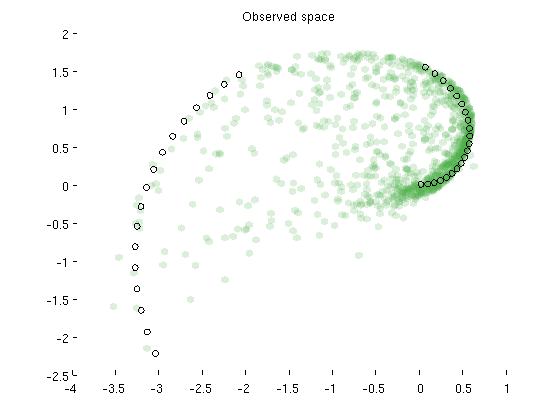
\includegraphics[width=\wmg,height=\hmg]{figures/first_demo_nocensor} 
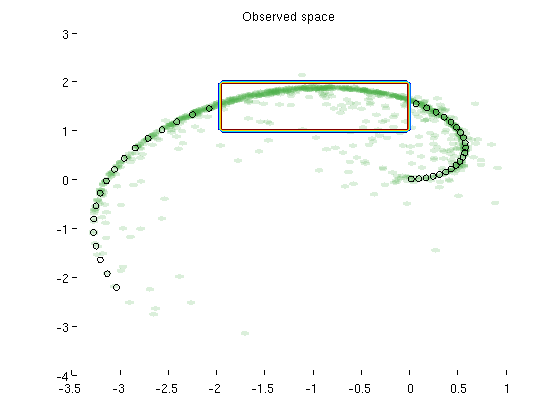
\includegraphics[width=\wmg,height=\hmg]{figures/second_demo_censor}
\end{tabular}
\caption{Modeling a truncated dataset.  Left:  Naively fitting a density manifold to the data.  Right:  When truncation is modeled explicitly, the model is not penalized for placing mass in censored regions, even though there is no mass there.}
\label{fig:synthetic}
\end{figure}



[Idea for a figure: plot the censored region in the latent space]

\subsection{Real data}



\section{Conclusions}

\subsubsection*{Acknowledgments}

We would like to thank Pushmeet Kohli for helpful discussions.

\bibliography{warped-censor}
\bibliographystyle{unsrt}

\end{document}
